%!TEX root = dippa.tex
%%% This file contains the results section of my master's thesis.
%%% Author: Viljami Aittomäki

\section{Results}

This section presents the results of performed analyses, and is structured as
follows. First, a short summary of quality control. The second subsection
present results from correlation analyses between variables of different data
types. Then results from the model simulations for projection predictive
variable selection are presented. Last, the performance of projection
prediction and lasso regression is assessed from a target prediction point of
view.




\subsection{Quality control}

Quality-control plots are presented in Appendix \ref{app:qc-plots}. Two
observations are worth noting. First, several genes have significant outliers
in the protein data (most notably the genes CDK1, ERRFI1, PIK3CA). This is
most apparent in the scaled data. Second, the miRNA microarrays have bimodal
distributions, and many miRNA variables are highly skewed towards very small
values. This is indicative of the generally low abundances of some miRNA molecules
and, although partly due to different preprocessing compared to the mRNA and
protein arrays, it raises suspicion of significant noise in the miRNA data.
The raw array data produced from Agilent array readers was not assessed here.

The first two principal components for each data type were plotted and are
shown in Figure \ref{fig:qc-pca}. No significant batch effect is visible. The
hierarchical clustering of samples (not shown) had a similar result.




\subsection{Correlation analysis}

Pearson correlations between variables from the different data types are shown in Figure
\ref{fig:correlations}. Protein-mRNA correlation is clearly higher for gene-matched pairs
(that is protein and mRNA expression corresponding to the same gene) than unmatched pairs,
and correlations for unmatched pairs are concentrated around zero, both expected
results. Notably, even the gene-matched correlations are quite low, with a
mean $\bar{\rho} \approx 0.37$. Using the squared correlation coefficient $\rho^2$ as a
measure of explained variance (although this has been criticized), the amount
of protein variance explained by the matched mRNA ranged from 0\% to 82\% with a mean of
21\%. This is in alignment with earlier results. 

\begin{figure}[!h]
  \centering
  \begin{subfigure}{.45\textwidth}
    \centering
    \includegraphics[width=1\linewidth]{figures/correlationPlots/protein-gene-correlation.pdf}
    \subcaption{ \label{fig:protein-gene-cor}}
  \end{subfigure}
  \begin{subfigure}{.45\textwidth}
    \centering
    \includegraphics[width=1\linewidth]{figures/correlationPlots/protein-mirna-correlation.pdf}
    \subcaption{ \label{fig:protein-mirna-cor}}
  \end{subfigure}
  \begin{subfigure}{.45\textwidth}
    %\centering
    \includegraphics[width=1\linewidth]{figures/correlationPlots/gene-mirna-correlation.pdf}
    \subcaption{ \label{fig:gene-mirna-cor}}
  \end{subfigure}

  \caption{Distributions of Pearson correlations between variables of different expression data types.
  The distributions are trimmed at the smallest and largest values.
  (a) Correlation between protein and mRNA pairs, where "matched" refers to correlating
  protein and mRNA from the same gene.
  (b) Correlation between protein and miRNA pairs, where "validated" refers to the gene
  being a validated target of the miRNA (according to Tarbase),
  and "random" to a randomly picked group of protein-miRNA pairs.
  (c) Correlation between mRNA and miRNA pairs,
  where grouping is the same as in (b).}
  \label{fig:correlations}
\end{figure}

Correlations between miRNAs and their validated target genes (fetched from
Tarbase) are mostly low with no preference towards negative (or positive)
values. There is virtually no difference in correlations between validated
targets and randomly picked gene-miRNA pairs, contrary to what might be
expected. This suggests that (Pearson) correlation of expression data is not a
suitable method for finding miRNA targets. It is possible that this is due to
the dataset used (and the noise in said data), however, as discussed in
Section \ref{expr-methods}, correlation has low power to detect weak
relationships and cannot capitalize on combinatorial effects. Therefore,
correlation was not used for target prediction in this work; poor
results with using correlation have been reported before
(see e.g. \citep{Muniategui2012}).




\subsection{Model simulations}

Simulations for the cross validation (to determine good model size) took
between 4 to 6 hours (\textbf{on a triton peXX machine}). Simulations for the
final projected models took between 2 to 45 minutes, depending on the chosen
model size. All parameters for all simulations had $\hat{R}^2 < 1.1$,
indicating good convergence of simulation chains \citep{Gelman2013}.

The
parameters for the model-size criterion, $\alpha$ and $\gamma$ had a
significant effect on the resulting model sizes (a plot of model-size
distributions is shown in appendix Figure \ref{fig:model-size-distribution}).
Values $\alpha = 0.50$ and
$\gamma = 0.2$ were chosen to keep models relatively sparse. This choice was,
however, largely subjective. Out of the 105 genes in the data, a projected model (where
at least one miRNA variable was included, and the model-size criterion was met
in under 200 variables) was then found for 74 genes. 
A table of properties for the projected models is presented in Appendix
\ref{app:full-model-table}.

Figure \ref{n-miRNAs-vs-R2} shows the number of miRNA variables included in
each projected model plotted against the number of significant miRNA
variables, the $R^2$ of the projected model, and the difference in $\bar{R}^2$
between the projected model and the gene-only model. Each point in each plot
corresponds to one gene, and smoothed curves were fitted using locally
weighted scatter plot smoothing (LOESS). A trend emerges, where including more
miRNA variables tends to achieve better performance up to a turning point --
around 28 miRNA variables -- after which larger models seem to perform
increasingly poorly. Similar plots were created with more strict model-size
thresholds ($\gamma$ and $\alpha$); the models were larger on
average, but an equal trend and turning point were observed (data not shown).

\begin{figure}[!h]
  \centering
  \includegraphics[height=11cm]{n_miRNAs_vs_R2.pdf}
  \caption{Size of final model compared to model goodness-of-fit. Plotted is the total number of chosen miRNA variables in each full model (N miRNAs) versus number of significant miRNA variables, R$^2$ of full model, and difference of $\bar{R}^2$ between full and gene only model ($\Delta\bar{R}^2$). Each point represents one model fitted for one gene. A small jitter has been added to the points to help visualize all of them. Curves were fitted with locally weighted scatter plot smoothing (LOESS) and shaded areas represent 95\% confidence interval. \label{n-miRNAs-vs-R2}}
\end{figure}

There could be several explanations for this trend. Firstly, the largest
models could simply be a result of the predictors not fitting the observed
variable well. This can result in a large model, because including more
predictors often makes the model fit asymptotically better -- both in the
sense of $R^2$ and generally also the predictive density, which was used as
the measure of fit for the variable-selection process. From a biological
perspective, this means that the mRNA and miRNA expression are not sufficient
to explain the protein expression; other factors, that the model does not
account for (e.g. protein degradation), possibly dominate.
Secondly, the marginal posterior of a single predictor can indicate
non-significance, while the joint posterior of several predictors combined
might still achieve significance. This would indicate that the effect of
miRNAs is only significant when acting simultaneously, a hypothesis that is
supported by experimental evidence, as discussed in section
\ref{microrna-function}.

Lasso regression produced models with at least one miRNA for 74 genes, out of
which only 57 were common to the ones found by projection prediction (PPVS).
For 18 of the lasso models, the mRNA expression variable was not included.
Figure \ref{fig:model-size} shows a comparison of model size distribution
and $\Delta\bar{R}^2$ between PPVS and lasso.

\begin{figure}[!h]
  \centering
  \begin{subfigure}{.45\textwidth}
    \centering
    \includegraphics[width=1\linewidth]{figures/R2comparison/n_miRNA_comparison.pdf}
  \end{subfigure}
  \begin{subfigure}{.45\textwidth}
    \centering
    \includegraphics[width=1\linewidth]{figures/R2comparison/R2_comparison.pdf}
  \end{subfigure}

  \caption{Comparison of model sizes and $\Delta\bar{R}^2$ for
      projection prediction (PPVS) and lasso regression.}
  \label{fig:model-size}
\end{figure}




\subsubsection{Target prediction performance}

Figure \ref{fig:venn} shows the number of putative targets
predicted by projection predictive variable
selection (PPVS) and lasso regression, as well as a comparison
of the distriburions of regression model sizes and $\Delta\bar{R}^2$'s
(compared to the gene-only model).

\begin{figure}
  \centering
  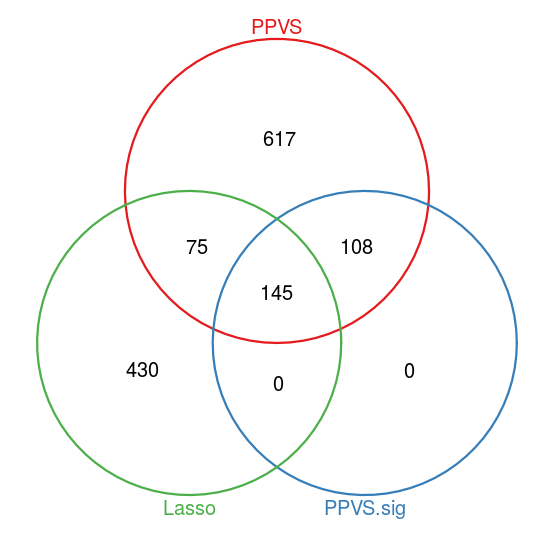
\includegraphics[width=.45\linewidth]{figures/compareModels/Venn_PPVS_PPVS-sig_Lasso.pdf}
  \caption{A Venn diagram showing the overlap of target predictions from both
  methods (including significant predictions from PPVS as their own group,
  shown left).}
  \label{fig:venn}
\end{figure}

Figure \ref{fig:scatter-ppvs-lasso} shows a comparison of the regression
coefficients from PPVS and lasso for targets predicted by both methods. There
were only 4 predicted targets for which the methods did not agree on the sign
of the coefficient, and all these coefficients were relatively small. PPVS
produced larger coefficients in general. Correlation for the coefficients was
fairly high ($0.86$).

\begin{figure}[htb]
  \centering
  \includegraphics[width=.6\linewidth]{figures/compareModels/PPVS_Lasso_coef_scatter.pdf}
  \caption{Scatter plot of miRNA regression coefficients from projection
  prediction (PPVS) and lasso for the 145 common targets predicted by both methods.
  Note that PPVS coefficients generally have greater magnitude. Triangles
  mark significant coefficients in PPVS. The gray
  line marks unity ($x=y$).}
  \label{fig:scatter-ppvs-lasso}
\end{figure}

Additionally, 206 negative interactions were listed for the data, i.e. gene-
miRNA pairs that showed no interaction in some experiment. PPVS and lasso had
similar performance in regards of discovering validated targets, with
approximately 17\% and 24\% of predicted targets being validated, respectively
(similarly, 17\% of significant predictions by PPVS were validated). Neither
method found any of the validated targets from breast cancer tissue. For both
methods, approximately half of the coefficients for both all predicted and
validated targets were positive, indicating upregulation by the miRNA, whereas
all of the discovered validated interactions were classified as downregulative
in Tarbase.
